\documentclass[11pt]{article}
\usepackage{amsmath,amssymb,amsthm,booktabs,geometry,graphicx,hyperref,natbib}
\geometry{margin=1in}
\hypersetup{hidelinks}
\setlength{\emergencystretch}{2em}
\allowdisplaybreaks
\newtheorem{proposition}{Proposition}
\newtheorem{corollary}{Corollary}
\title{Green Subsidies, Public Infrastructure, and Product-Market Rivalry: When Cross-Instrument Responses Reverse}
\author{Ryota Matsuki\\
Independent Researcher\\
Matsuyama, Ehime, Japan\\
Corresponding author: \texttt{ryota.matsuki@gmail.com}\\
ORCID: \href{https://orcid.org/0009-0005-2329-531X}{0009-0005-2329-531X}}
\date{}

\begin{document}
\maketitle

\begin{abstract}
How does product-market rivalry alter the infrastructure response to a rival jurisdiction's green-investment subsidy when governments adjust subsidies and productive public inputs simultaneously? We study a three-stage game in which governments choose these two instruments, firms choose conventional cost-reducing and green investment, and differentiated producers compete. Under explicit sufficient conditions, product substitutability uniquely reverses the cross-instrument infrastructure best response. A Schur-complement decomposition shows why the direct infrastructure incentive may turn positive while the government's simultaneous optimal subsidy adjustment still induces infrastructure contraction. On a fixed-environmental-primitives slice, an exact interior comparative-static result identifies a critical investment-feedback strength: below it the response stays negative, whereas above it a unique rivalry threshold emerges and falls as investment becomes more flexible. We separately solve nonnegative duopoly, limit-pricing, and monopoly continuations and certify that the canonical rational witness supports a true SPNE of the full nonnegative-action game on an open primitive neighborhood. Removing conventional investment eliminates the reversal at the same remaining canonical primitives, although this investment margin is not universally necessary for switching. The mechanism also survives locally under differentiated Bertrand competition and partial local capture of firm surplus. The results characterize strategic policy reactions, not a general welfare ordering or an emissions-reduction guarantee.
\end{abstract}

\noindent\textbf{Keywords:} green industrial policy; interjurisdictional competition; public infrastructure; green investment; oligopoly\\
\textbf{JEL codes:} H23, H71, L13, Q55, Q58, R58

\section{Introduction}
\label{sec:introduction}

Green industrial policy is increasingly place based. Governments can support firm-level decarbonizing investment, and policy packages can also include shared inputs---clean-power access, utility networks, ports, industrial land, grid capacity, and related infrastructure---that affect local production conditions. Japan's GX Strategic Area framework illustrates this policy architecture by combining place-based industrial-cluster and infrastructure measures with a separate firm-facing investment-support channel \citep{METIGX2026,METIGXSubsidy2026}. Subnational decarbonization objectives can also be policy relevant; the OECD documents a substantial subnational role in Japan's green transition \citep{OECDJapan2025}. These choices operate in markets where firms compete across jurisdictional boundaries. A policy adopted in one region can therefore change not only emissions and local investment, but also the product-market position of firms located elsewhere.

This raises a cross-instrument public-finance question. Suppose a rival jurisdiction increases firm-facing green support. Should a local government match that support, retreat, or respond through a different instrument? The distinction matters because a rival subsidy may either crowd out local infrastructure provision or induce a jurisdiction to reinforce shared productive capacity. We show that the sign of the infrastructure response can change with product-market substitutability when firms choose both conventional cost-reducing investment and green investment. Throughout, ``switching'' refers to this reversal in the direction of the cross-instrument response, not to discrete adoption of one instrument instead of another.

The contribution is deliberately narrower than the ingredients of the model. Multi-instrument jurisdictional competition and cross-instrument reactions are already central to the fiscal-competition literature; \citet{HauptmeierMittermaierRincke2012} study business taxes and productive public inputs, while \citet{BenassyQuereGobalrajaTrannoy2007} analyze tax and public-input competition more generally. \citet{MoritaOkoshi2025} show that fiscal competition and infrastructure can interact with Cournot competition and threshold effects. Their central comparison concerns how fiscal competition changes infrastructure investment in an FDI setting; our object instead is the sign of the infrastructure best-response derivative to a rival firm-facing subsidy with fixed-location incumbents and endogenous conventional and green investment. Simultaneous conventional and green R\&D is also known \citep{StrandholmEspinolaMunoz2025}. We therefore do not claim novelty for policy multiplicity, infrastructure competition, dual investment, or threshold effects as such. The surviving theorem-level distinction is that, over a certified nonempty global-SPNE region, product substitutability uniquely reverses the sign of the same local infrastructure response to a rival green-investment subsidy; at the canonical remaining primitives, a matched benchmark without conventional investment lacks that reversal.

We study two jurisdictions, each hosting one fixed-location firm. Local governments first choose a firm-specific green-investment subsidy and productive green public infrastructure. Firms then choose conventional cost-reducing investment and green investment, followed by differentiated Cournot competition. Green investment can both reduce emissions and affect productivity, while infrastructure can affect production costs and territorial emissions. The model contains no hard government budget linking the two policies and no firm-level investment constraint linking conventional and green investment.

The main result is a competition-induced sign reversal. On an interior duopoly branch, primitive sufficient conditions reduce the cross-instrument best-response derivative to the sign of a quartic polynomial in $\theta^2$. Bernstein-basis conditions make that polynomial strictly decreasing, yielding a unique threshold $\theta^*$. The global-equilibrium issue is treated separately: with nonnegative policies, investments, and quantities, sufficiently aggressive policies can change market structure. We therefore solve the duopoly, limit-pricing-kink, and monopoly continuations and show that the canonical rational witness supports a true global policy SPNE on a nonempty open neighborhood. At that witness, $\theta^*\simeq0.774$.
Figure~\ref{fig:threshold-response} previews the sign reversal and contrasts it with the matched benchmark without conventional competitive investment.

The mechanism can be described more sharply without treating the model's ingredients as novel. A rival subsidy changes quantities and firm investment; the government then evaluates both a direct infrastructure incentive and an indirect adjustment through its own subsidy. In the canonical example, the infrastructure-only response turns positive at product substitutability of about $0.426$, but the simultaneous two-policy response remains negative until about $0.774$. Thus adjusting the second instrument can reverse the sign of the policy reaction, not merely its magnitude. On the fixed-environmental-primitives slice, we further prove that total firm investment flexibility must exceed a unique boundary $R_c\simeq0.140$ for an interior response reversal to occur, and that the switching threshold falls as investment flexibility rises above this boundary. These statements are conditional on the interior continuation; the separate global-SPNE certificate establishes their equilibrium interpretation for the canonical witness and its certified neighborhood.

The investment-flexibility comparison gives the nested benchmark a more systematic role. Holding the remaining canonical primitives fixed, the no-conventional-investment limit has $R=0.045$, below the critical value, while the full model has $R=0.295$, above it. This is not a universal necessity theorem: at different environmental primitives, the no-conventional-investment model itself can exhibit switching. When green investment has no productivity effect, moreover, the rival-subsidy product-market transmission vanishes.

The welfare analysis is secondary. Decentralized governments do not internalize the effects of their policies on rival-region consumer surplus, producer surplus, and territorial emissions objectives, so decentralized and coordinated decisions generally differ. In the canonical example coordination raises total model welfare and increases the fiscal weight of infrastructure, but it also raises output and territorial emissions. The result is therefore a second-best regional-welfare comparison, not a theorem that coordination necessarily produces lower emissions.

The institutional mapping remains deliberately limited. The Japanese programs cited above motivate the coexistence of place-based productive infrastructure and firm-facing green investment support, but they do not imply that Japanese local governments literally control both instruments as specified here. The model is a stylized interjurisdictional-policy game rather than a literal mapping of legal authority or financing incidence.

The remainder of the paper proceeds as follows. Section~\ref{sec:model} presents the model and action sets. Section~\ref{sec:equilibrium} solves the interior and boundary continuations. Section~\ref{sec:results} derives the switching threshold and matched benchmark. Section~\ref{sec:welfare} studies coordination. Section~\ref{sec:robustness} considers differentiated Bertrand competition and partial local ownership. Section~\ref{sec:institutional} develops empirical predictions and the institutional mapping. Section~\ref{sec:literature} places the result in the related literature, and the final sections discuss scope and conclude.

\section{Model}
\label{sec:model}

There are two jurisdictions, indexed by $i\in\{A,B\}$, and one incumbent manufacturing firm in each jurisdiction. Plant locations are fixed. The model is intended to capture industries in which production is geographically anchored but product-market competition is broader than the jurisdiction itself. Information is complete and all primitives are common knowledge.

\subsection{Timing and action sets}

The game has three stages. In Stage 1, local governments simultaneously choose a firm-specific green-investment subsidy $s_i\geq0$ and shared green public infrastructure $h_i\geq0$. In Stage 2, firms simultaneously choose conventional cost-reducing investment $x_i\geq0$ and green investment $g_i\geq0$. In Stage 3, firms compete in nonnegative quantities $q_i\geq0$. We solve for a subgame-perfect Nash equilibrium by backward induction. Because sufficiently aggressive policies can change the set of active firms, the continuation game is defined on the full nonnegative action space rather than only on the two-active-firm branch.

\subsection{Product market}

A representative consumer has gross utility
\begin{equation}
V(q_A,q_B)
=a(q_A+q_B)-\frac12(q_A^2+q_B^2)-\theta q_Aq_B,
\label{eq:grossutility}
\end{equation}
which implies inverse demand
\begin{equation}
p_i=a-q_i-\theta q_j,
\qquad i\neq j,
\label{eq:inverse-demand}
\end{equation}
with $0\leq\theta\leq1$. We maintain $a>c$, so the baseline net market intercept used below satisfies $m\equiv a-c>0$. This restriction rules out a separate both-inactive baseline region in the continuation map; it is satisfied strictly at the canonical witness and on a sufficiently small primitive neighborhood. The parameter $\theta$ measures product substitutability and hence the intensity of product-market rivalry. Consumer surplus is
\begin{equation}
CS=\frac12(q_A^2+q_B^2)+\theta q_Aq_B.
\label{eq:cs}
\end{equation}

\subsection{Technology, investment, and emissions}

Firm $i$ has marginal cost
\begin{equation}
c_i=c-x_i-\mu g_i-\nu h_i.
\label{eq:mc}
\end{equation}
Conventional investment $x_i$ raises productivity. Green investment $g_i$ reduces emissions and, when $\mu>0$, also improves competitiveness. Shared green infrastructure $h_i$ is a local public input that can lower firms' marginal cost at rate $\nu>0$. Investment costs are separable and quadratic,
\begin{equation}
C_i(x_i,g_i)
=\frac{k_x}{2}x_i^2+\frac{k_g}{2}g_i^2,
\qquad k_x,k_g>0.
\label{eq:investment-cost}
\end{equation}
There is no exogenous investment budget linking $x_i$ and $g_i$; any interaction between the two investments is generated endogenously through the product market.

Firm $i$'s profit is
\begin{equation}
\pi_i
=(p_i-c_i)q_i
-\frac{k_x}{2}x_i^2
-\frac{k_g}{2}g_i^2
+s_i g_i.
\label{eq:profit}
\end{equation}
Territorial emissions are
\begin{equation}
E_i=e q_i-\beta g_i-\xi h_i,
\qquad e,\beta>0,\quad \xi\geq0.
\label{eq:emissions}
\end{equation}
The term $e q_i$ captures the scale effect of production, while $\beta g_i$ and $\xi h_i$ capture private and public abatement channels.

\subsection{Local-government objective}

The local government values one half of integrated-market consumer surplus, local producer surplus, and progress toward a territorial emissions target. Its objective is
\begin{equation}
W_i
=\frac12CS+PS_i-\frac{\kappa}{2}h_i^2
-\frac d2(E_i-\bar E_i)^2,
\qquad \kappa,d>0,
\label{eq:government-welfare}
\end{equation}
where producer surplus is defined globally as
\begin{equation}
PS_i=(p_i-c_i)q_i-\frac{k_x}{2}x_i^2-\frac{k_g}{2}g_i^2.
\label{eq:producer-surplus}
\end{equation}
On an active interior Cournot branch, $p_i-c_i=q_i$, so \eqref{eq:producer-surplus} reduces to $q_i^2-(k_x/2)x_i^2-(k_g/2)g_i^2$. The global definition remains valid when a firm is inactive. The subsidy payment $s_i g_i$ is an intrajurisdictional transfer and therefore cancels from regional welfare in the full-local-capture baseline. The quadratic emissions term should be interpreted as a reduced-form loss from deviating from a delegated or territorial decarbonization objective, not as local physical climate damages from carbon emissions.

\subsection{Regularity and equilibrium scope}

Define
\begin{equation}
R\equiv\frac1{k_x}+\frac{\mu^2}{k_g}.
\label{eq:R}
\end{equation}
We impose the convenient sufficient condition
\begin{equation}
R<\frac34.
\label{eq:regularity}
\end{equation}
This condition is stronger than necessary, but it guarantees the relevant firm-stage regularity and nonsingularity conditions for all $\theta\in[0,1]$. The comparative statics in Section~\ref{sec:results} are derived on the interior two-active-firm branch, where the government own-policy Hessian is negative definite. Separately, the global-equilibrium verification compares that branch with the nonnegative-policy kink and monopoly continuations. For the canonical rational witness, the interior policy candidate is a true global policy Nash equilibrium for every $\theta\in[0,1]$, and all inequalities hold strictly on a nonempty neighborhood of primitives. Thus the reported local best-response derivative is locally the derivative of the true global best response, not merely of a stationary branch.
\section{Equilibrium Characterization}
Let $D\equiv 4-\theta^2$. At the Cournot stage, $p_i-c_i=q_i$. Backward induction yields
\[
x_i^*=\frac{4q_i}{Dk_x},\qquad
g_i^*=\frac{4\mu q_i/D+s_i}{k_g}.
\]
Define
\[
R\equiv\frac1{k_x}+\frac{\mu^2}{k_g},\qquad
\lambda\equiv\frac{4R}{D},\qquad
y_i\equiv\frac{\mu}{k_g}s_i+\nu h_i.
\]
A convenient sufficient regularity condition is $R<3/4$. The reduced output system is
\[
(D-2\lambda)q_i+\theta\lambda q_j=(2-\theta)(a-c)+2y_i-\theta y_j.
\]
All manuscript algebra must be checked against the symbolic verification scripts in this repository.

\section{Main Results}
\label{sec:results}

The central object is the response of jurisdiction $A$'s infrastructure policy to jurisdiction $B$'s firm-specific green subsidy,
\[
\frac{\partial h_A^{BR}}{\partial s_B}.
\]
The question is not whether governments use multiple instruments---that possibility is well established---but whether stronger product-market rivalry can change the sign of this cross-instrument response once firms' conventional and green investments are jointly endogenous.

\subsection{A general cross-instrument decomposition}

Let
\[
H_A=
\begin{pmatrix}
W_{s_As_A}&W_{s_Ah_A}\\
W_{s_Ah_A}&W_{h_Ah_A}
\end{pmatrix}
\]
be government $A$'s own-policy Hessian on an interior duopoly branch. Differentiating its two first-order conditions with respect to $s_B$ gives
\begin{equation}
\begin{pmatrix}
\partial s_A^{BR}/\partial s_B\\[2pt]
\partial h_A^{BR}/\partial s_B
\end{pmatrix}
=-H_A^{-1}
\begin{pmatrix}
W_{s_As_B}\\W_{h_As_B}
\end{pmatrix}.
\label{eq:br-ift}
\end{equation}
Under strict concavity, $\det H_A>0$, so
\begin{equation}
\frac{\partial h_A^{BR}}{\partial s_B}
=\frac{W_{s_Ah_A}W_{s_As_B}-W_{s_As_A}W_{h_As_B}}{\det H_A}.
\label{eq:cross-instrument-general}
\end{equation}
The numerator combines a direct cross effect, $W_{h_As_B}$, with an indirect term transmitted through the interaction between the local government's two instruments. A sign reversal is possible when product-market rivalry changes their relative strength. An equivalent Schur-complement representation makes the policy-adjustment channel explicit:
\begin{equation}
\frac{\partial h_A^{BR}}{\partial s_B}
=-\frac{
W_{h_As_B}-W_{h_As_A}W_{s_As_B}/W_{s_As_A}
}{
W_{h_Ah_A}-W_{h_As_A}^{\,2}/W_{s_As_A}
}.
\label{eq:schur-policy}
\end{equation}
Negative definiteness of $H_A$ makes the denominator strictly negative. Thus the sign is determined by the direct infrastructure cross effect \emph{net of} the adjustment permitted through the government's own subsidy. If the own subsidy were instead held fixed, the infrastructure-only response would be $-W_{h_As_B}/W_{h_Ah_A}$. Equation~\eqref{eq:schur-policy} is an algebraic decomposition of the established two-policy reaction system, not a novel comparative-statics theorem by itself.

For $\mu>0$ in the model of Sections~\ref{sec:model}--\ref{sec:equilibrium}, symbolic reduction yields a positive function $\Omega(\theta)$ and a quartic
\begin{equation}
P(u)=A_4u^4+A_3u^3+A_2u^2+A_1u+A_0,
\qquad u\equiv\theta^2,
\label{eq:P-def}
\end{equation}
such that
\begin{equation}
\frac{\partial h_A^{BR}}{\partial s_B}
=-\Omega(\theta)P(\theta^2),
\qquad \Omega(\theta)>0
\quad\text{for }\theta\in(0,1].
\label{eq:P-sign}
\end{equation}
The coefficients $A_j$ are explicit functions of the primitives $(k_x,k_g,\mu,\nu,d,e,\beta,\xi)$; intercept terms such as $a-c$ and the emissions-target level $\bar E_i$ drop out of the best-response slope. Appendix~\ref{app:proofs} records the reduction and the repository contains an independent symbolic verification. The case $\mu=0$ is treated separately in Corollary~\ref{cor:mu-zero}, because the rival subsidy then has no product-market transmission through green investment.

Define the Bernstein coefficients of $P'$ on $[0,1]$ as
\begin{align}
B_0&=A_1,\\
B_1&=A_1+\frac23A_2,\\
B_2&=A_1+\frac43A_2+A_3,\\
B_3&=A_1+2A_2+3A_3+4A_4.
\label{eq:bernstein-derivative}
\end{align}

\begin{proposition}[Unique instrument-switching threshold]
\label{prop:threshold}
Suppose $\mu>0$, the firm-stage regularity and government strict-concavity conditions hold on an interior duopoly best-response branch, and suppose
\begin{equation}
P(0)>0,\qquad P(1)<0,
\qquad B_0,B_1,B_2,B_3<0.
\label{eq:threshold-conditions}
\end{equation}
Then there exists a unique $\theta^*\in(0,1)$ such that
\begin{equation}
0<\theta<\theta^*
\quad\Longrightarrow\quad
\frac{\partial h_A^{BR}}{\partial s_B}<0,
\end{equation}
and
\begin{equation}
\theta^*<\theta\leq1
\quad\Longrightarrow\quad
\frac{\partial h_A^{BR}}{\partial s_B}>0.
\end{equation}
If, in addition, that interior branch is the true global policy best response on an open neighborhood, the same derivative is the derivative of the global best response there.
\end{proposition}

The proof is simple once the equilibrium has been reduced to \eqref{eq:P-sign}. The conditions $B_0,\ldots,B_3<0$ imply $P'(u)<0$ throughout $[0,1]$ because the cubic Bernstein basis is nonnegative on that interval. Combined with $P(0)>0>P(1)$, this yields a unique root $u^*\in(0,1)$ and hence $\theta^*=\sqrt{u^*}$. At $\theta=0$ the cross-jurisdictional response is zero rather than negative.

\subsection{Economic mechanism}

A higher $s_B$ raises firm $B$'s green investment. When $\mu>0$, that investment also affects marginal production cost and product-market quantities. The resulting business-stealing effect changes $A$'s output and both of its endogenous investment choices. The feedback strength is summarized by
\[
R=\frac1{k_x}+\frac{\mu^2}{k_g}.
\]
Product substitutability changes how this investment feedback propagates through quantities, but the final government response is not a pure competitiveness-preservation effect. Equation~\eqref{eq:cross-instrument-general} combines consumer-surplus, producer-surplus, territorial-target, and within-government policy-interaction terms.

At the canonical global-SPNE point $\theta=.9$, the direct cross derivative is
\[
W_{h_As_B}
=0.001638_{\,CS}
-0.039629_{\,PS}
+0.046078_{\,\text{target}}
=0.008087.
\]
Moreover, $E_{A,h_A}\simeq0.952>0$ while $E_{A,s_B}\simeq-0.0242$. Thus a rival subsidy lowers local output and territorial emissions, which in this calibration relaxes part of the target-loss consequence of an infrastructure expansion even though infrastructure raises local emissions on net through its scale effect. The switching result should therefore be read as a composite strategic response rather than as evidence that one single channel dominates generally.

The interior reduced system also implies that rival policies enter jurisdiction $A$ through
\[
y_B=\frac{\mu}{k_g}s_B+\nu h_B.
\]
Hence, whenever the same interior branch applies,
\begin{equation}
\frac{\partial z_A^{BR}}{\partial h_B}
=\frac{\nu k_g}{\mu}
\frac{\partial z_A^{BR}}{\partial s_B},
\qquad z_A\in\{s_A,h_A\}.
\label{eq:rival-policy-proportionality}
\end{equation}
The rival-subsidy shock is therefore a convenient cross-instrument normalization, not a uniquely identified transmission channel.

\subsection{Canonical global-SPNE witness}

Set
\[
k_x=4,\quad k_g=18,\quad \mu=0.9,\quad \nu=1.2,
\quad \kappa=0.8,
\]
\[
d=2,\quad e=1.1,\quad \beta=1.7,\quad \xi=0.1,
\quad a-c=2,\quad \bar E_i=0.
\]
A convenient positive rescaling of the switching polynomial is
\begin{align}
\widetilde P(u)=
&602500u^4-8101550u^3+39588109u^2\\
&-74143042u+31863144.
\label{eq:witness-P}
\end{align}
It has exactly one root in $[0,1]$,
\[
u^*=0.5987732279\ldots,
\qquad
\theta^*=0.7738043861\ldots.
\]
The full nonnegative-policy continuation in Section~\ref{sec:equilibrium} verifies that the symmetric interior policy candidate is a true global policy Nash equilibrium throughout $\theta\in[0,1]$ for this rational witness. The comparison with the best kink/monopoly challenger is strict, so the property survives on a nonempty open neighborhood of primitives.

\begin{figure}[!t]
\centering
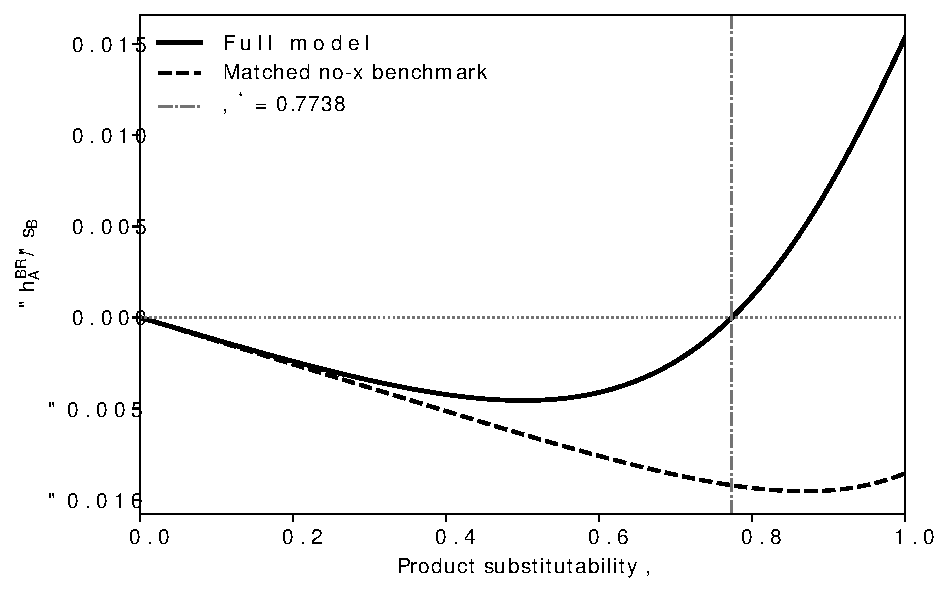
\includegraphics[width=0.72\textwidth]{figures/figure1_threshold_response.pdf}
\caption{Canonical cross-instrument infrastructure response. The solid line is the full model and the dashed line is the matched no-conventional-investment benchmark at the same remaining canonical primitives. The horizontal line marks zero and the vertical marker indicates $\theta^*=0.7738043861\ldots$. The full-model response crosses zero once, whereas the matched no-$x$ response remains negative for all $\theta\in(0,1]$.}
\label{fig:threshold-response}
\end{figure}

Figure~\ref{fig:threshold-response} plots the canonical cross-infrastructure response over the full rivalry range. The response is initially negative, becomes more negative at intermediate rivalry, and then rises through zero exactly once at $\theta^*=0.7738043861\ldots$. Thus the result is a threshold sign change rather than a globally monotone increase in the response as product-market rivalry intensifies.

At $\theta=0.9$ the symmetric equilibrium is
\[
(s^*,h^*)=(2.0594,0.7443),
\]
with
\[
(q,x,g,E)=(1.1842,0.3712,0.1887,0.9075).
\]
Table~\ref{tab:br-slopes} reports representative values of the two best-response slopes on either side of the threshold plotted in Figure~\ref{fig:threshold-response}.

\begin{table}[htbp]
\centering
\caption{Response of jurisdiction $A$ to a higher rival green subsidy}
\label{tab:br-slopes}
\begin{tabular}{lcc}
\toprule
& $\theta=0.5$ & $\theta=0.9$\\
\midrule
$\partial s_A^{BR}/\partial s_B$ & $-0.02590$ & $-0.02749$\\
$\partial h_A^{BR}/\partial s_B$ & $-0.00455$ & $+0.00711$\\
\bottomrule
\end{tabular}
\end{table}

\subsection{Policy adjustment and investment-feedback boundary}
\label{subsec:investment-boundary}

The Schur decomposition yields a sharper comparison at the canonical witness. Holding $s_A$ fixed, the infrastructure-only response $-W_{h_As_B}/W_{h_Ah_A}$ changes from negative to positive at $\theta_D\simeq0.4257368$. When $s_A$ can adjust jointly with $h_A$, the corresponding response does not become positive until $\theta^*\simeq0.7738044$. On $(\theta_D,\theta^*)$, therefore, the direct infrastructure incentive favors expansion, yet the government's simultaneous optimal subsidy adjustment makes its infrastructure best response contract. These are distinct \emph{response experiments} within the same reduced government objective, not a comparison of two globally solved policy games. The exact signs and uniqueness of both thresholds are verified in Appendix~\ref{app:investment-boundary}.

The contribution of conventional investment can be expressed more systematically than a single no-$x$ comparison. Keep $(k_g,\mu,\nu,\kappa,d,e,\beta,\xi,m,\bar E)$ at their canonical values, while allowing $k_x$ to vary, and let
\[
r\equiv R=\frac1{k_x}+\frac{\mu^2}{k_g}
\in\left[\frac9{200},\frac{59}{200}\right].
\]
The lower endpoint is the no-conventional-investment limit; the upper endpoint has $k_x=4$. The relevant cross-response numerator has the sign of the polynomial $Q(r,u)$ displayed in Appendix~\ref{app:investment-boundary}, with $u=\theta^2$.

\begin{proposition}[Investment flexibility and the switching boundary on the interior branch]
\label{prop:investment-boundary}
On the active-duopoly continuation and the one-parameter primitive slice just specified, the government own-policy Hessian is negative definite for every $r\in[9/200,59/200]$ and $\theta\in[0,1]$. There is a unique
\[
r_c\in\left(\frac9{200},\frac{59}{200}\right),
\qquad
2198800r_c^2-4239456r_c+549747=0,
\qquad r_c\simeq0.1398123,
\]
such that the infrastructure response to a rival subsidy is negative for all $\theta\in(0,1]$ when $r<r_c$; it is negative for $\theta\in(0,1)$ and zero at $\theta=1$ when $r=r_c$; and it switches exactly once from negative to positive for $\theta\in(0,1]$ when $r>r_c$. In the switching region, the threshold $\theta^*(r)$ strictly decreases with $r$.
\end{proposition}

The result isolates an economically interpretable boundary in \emph{investment flexibility}: with the remaining environmental primitives held fixed, sufficiently responsive conventional cost-reducing investment changes the qualitative strategic policy reaction, rather than simply shifting its magnitude. Because $r$ also includes the green-investment productivity term, this statement is a fixed-primitives comparative static, not a claim that conventional investment is universally necessary for switching. Indeed the separately verified no-$x$, $\beta=1.3$ example still switches. Proposition~\ref{prop:investment-boundary} is an \emph{interior-branch} result throughout the displayed $r$ interval; the existing cross-regime global-SPNE certificate applies to the canonical upper endpoint and its certified open neighborhood, not automatically to every $r$ in this interval.

\subsection{Matched benchmark without conventional competitive investment}

Consider the nested benchmark in which conventional investment is removed, equivalently $1/k_x\rightarrow0$. Let $\bar P(u)$ denote the resulting cross-instrument polynomial and let $C_0,\ldots,C_4$ be its degree-four Bernstein coefficients.

\begin{proposition}[Matched no-conventional-investment benchmark]
\label{prop:no-x}
Suppose the benchmark is interior and strictly concave. If
\[
C_0,C_1,C_2,C_3,C_4>0,
\]
then
\[
\frac{\partial h_A^{BR}}{\partial s_B}<0
\qquad\forall\theta\in(0,1].
\]
Hence the sign reversal is absent from that benchmark region.
\end{proposition}

For the canonical parameter values, the no-$x$ expression is proportional to
\begin{equation}
602500u^2-3281550u+3486659,
\label{eq:no-x-witness}
\end{equation}
which is strictly positive on $u\in[0,1]$. The full and nested models therefore generate qualitatively different best-response networks at the same canonical environmental and policy primitives. For this matched no-$x$ canonical vector, a separate exact analysis of the full nonnegative continuation also verifies the interior policy candidate against all kink- and monopoly-inducing deviations for every $\theta\in[0,1]$. Consequently the matched comparison is not merely between formal interior stationary points; both canonical systems have globally valid policy equilibria over the full rivalry interval. This extra global guarantee applies to this matched canonical vector, not to arbitrary benchmark primitives.

The dashed curve in Figure~\ref{fig:threshold-response} visualizes this matched benchmark separation: at the same canonical remaining primitives, the no-$x$ response stays below zero for all positive rivalry levels.

This is a matched benchmark separation, not a universal necessity result. Holding the other primitives fixed but changing $\beta$ to $1.3$ produces a verified no-$x$ global-equilibrium example in which the response is negative at $\theta=.9$ and positive at $\theta=1$. Conventional investment can therefore create a reversal that is absent under the matched canonical benchmark, but it is not necessary for every possible reversal.

\begin{corollary}[Competitiveness link]
\label{cor:mu-zero}
If $\mu=0$, green investment has no effect on product-market competitiveness. A rival subsidy then changes rival abatement but not rival output through this channel, and
\[
\frac{\partial s_A^{BR}}{\partial s_B}
=
\frac{\partial h_A^{BR}}{\partial s_B}=0.
\]
\end{corollary}

Finally, the threshold has economically interpretable local comparative statics. Around the canonical region,
\[
\frac{\partial\theta^*}{\partial\nu}<0,
\qquad
\frac{\partial\theta^*}{\partial k_x}>0.
\]
Thus, locally, switching occurs at weaker product-market rivalry when shared infrastructure is more productive or when firms can adjust conventional competitive investment more flexibly. These derivatives are local results rather than global monotonicity claims.
\section{Welfare and Coordination}
\label{sec:welfare}

The main contribution concerns strategic instrument switching, not a generic decentralization inefficiency. Nevertheless, the model delivers a useful welfare benchmark because the decentralized governments internalize different margins from a coordinated policymaker.

Let the coordinated policy vector maximize
\begin{equation}
\max_{s_A,h_A,s_B,h_B\geq0}\;W_A+W_B.
\label{eq:planner}
\end{equation}
For any policy $z_A\in\{s_A,h_A\}$, the difference between the coordinated and decentralized first-order conditions can be written as
\begin{equation}
\Omega_{z_A}^{W}
\equiv
\frac{\partial W_B}{\partial z_A}.
\label{eq:welfare-wedge-def}
\end{equation}
Using the structure of $W_B$,
\begin{equation}
\Omega_{z_A}^{W}
=
\frac12\frac{\partial CS}{\partial z_A}
+
\frac{\partial PS_B}{\partial z_A}
-
d(E_B-\bar E_B)\frac{\partial E_B}{\partial z_A}.
\label{eq:welfare-wedge}
\end{equation}
The wedge therefore contains three real cross-jurisdictional effects: consumer-surplus effects, producer-surplus/business-stealing effects, and emissions-target effects. The welfare comparison is not generated by subsidy transfers alone.

The sign of each wedge is parameter dependent, so the theory does not imply a global ranking of each decentralized policy instrument relative to its coordinated counterpart. In particular, the rivalry threshold for a \emph{best-response derivative} in Proposition~\ref{prop:investment-boundary} is not a threshold for efficient provision: $\partial h_A^{BR}/\partial s_B$ and the coordination wedge $\partial W_B/\partial h_A$ are different derivatives. Therefore neither a positive strategic infrastructure response nor a lower investment-feedback threshold establishes underprovision of infrastructure, higher total welfare, or lower emissions. This distinction is retained rather than imposing an unsupported welfare-ordering theorem. For the canonical parameter vector, Table~\ref{tab:welfare} reports the symmetric decentralized global-SPNE policy and the symmetric coordinated active-duopoly benchmark. The coordinated entries are an interior benchmark, not a separate global-equilibrium theorem for the planner problem.

Because $s$ is a subsidy rate while $h$ is an infrastructure quantity, the ratio $h/(s+h)$ has no meaningful unit interpretation and is not used. For a descriptive fiscal-composition measure, define
\begin{equation}
\phi_h
\equiv
\frac{\kappa h^2/2}{s g+\kappa h^2/2}.
\label{eq:fiscal-infra-share}
\end{equation}
This compares subsidy outlay $sg$ with the infrastructure resource/outlay term in common units. It is not a welfare share because the subsidy transfer cancels from baseline regional welfare.

\begin{table}[htbp]
\centering
\small
\caption{Decentralized and coordinated policies in the canonical witness}
\label{tab:welfare}
\begin{tabular}{ccccccc}
\toprule
$\theta$ & $s^{NE}$ & $h^{NE}$ & $\phi_h^{NE}$ & $s^{C}$ & $h^{C}$ & $\phi_h^{C}$\\
\midrule
0.60 & 2.941 & 1.143 & 0.417 & 7.003 & 4.597 & 0.676\\
0.774 & 2.445 & 0.941 & 0.403 & 5.407 & 3.692 & 0.685\\
0.90 & 2.059 & 0.744 & 0.363 & 4.525 & 3.199 & 0.692\\
1.00 & 1.709 & 0.524 & 0.281 & 3.923 & 2.867 & 0.698\\
\bottomrule
\end{tabular}
\begin{flushleft}\footnotesize
Notes: $C$ denotes the symmetric coordinated solution on the active-duopoly branch. The table is an illustration, not a global policy-ordering theorem.
\end{flushleft}
\end{table}

At $\theta=0.9$, total welfare is approximately $2.187$ in the decentralized global-SPNE equilibrium and $3.720$ at the symmetric coordinated active-duopoly benchmark. The fiscal infrastructure share rises from $0.363$ to $0.692$. However, coordination also raises each region's output from approximately $1.184$ to $2.397$ and territorial emissions from approximately $0.907$ to $1.634$.

This last comparison is important for interpretation. Coordination is not an emissions-reduction theorem. The coordinated policymaker internalizes cross-jurisdictional consumer-surplus, producer-surplus, and territorial-target effects, and in the canonical example the production gain is large enough that the coordinated solution tolerates higher territorial emissions. The exercise is therefore a second-best regional-welfare comparison rather than a claim that more coordination necessarily produces greener physical outcomes.

Nor should these numbers be interpreted as a recommendation for globally maximizing carbon policy. The model's emissions term represents territorial or delegated decarbonization objectives. A global climate externality depending on $E_A+E_B$ would introduce an additional coordination motive. We deliberately leave that global-damage extension outside the baseline so that the paper isolates the strategic interaction between local green industrial policy and product-market rivalry.

\section{Robustness and Scope}
\label{sec:robustness}

The switching result is not intended to be universal. Its content is that a cross-instrument sign reversal exists under economically interpretable conditions and, in the canonical Cournot region, is supported by a true global policy SPNE. This section asks whether the local sign mechanism survives alternative product-market competition and incomplete local ownership, and how the environmental-target motive affects the shape of the response. These exercises are deliberately narrower than the baseline global-equilibrium certificate.

\subsection{Differentiated Bertrand competition}

Retain the quadratic utility in \eqref{eq:grossutility} but let firms choose prices in the final stage. The corresponding direct demand is
\begin{equation}
q_i
=\frac{a(1-\theta)-p_i+\theta p_j}{1-\theta^2},
\qquad 0\leq\theta<1.
\label{eq:bertrand-demand}
\end{equation}
The price first-order condition implies
\begin{equation}
p_i-c_i=(1-\theta^2)q_i,
\label{eq:bertrand-margin}
\end{equation}
so operating profit is $(1-\theta^2)q_i^2$. Backward induction through the investment stage gives
\begin{equation}
x_i^B=\frac{\eta(\theta)q_i}{k_x},
\qquad
g_i^B=\frac{\eta(\theta)\mu q_i+s_i}{k_g},
\end{equation}
where
\begin{equation}
\eta(\theta)=\frac{2(2-\theta^2)}{4-\theta^2}.
\end{equation}
The reduced interior government problem remains linear-quadratic.

Using the same primitive parameter vector as the Cournot witness, the Bertrand cross-infrastructure response is negative at $\theta=.3$ and positive at $\theta=.5$:
\[
\left.\frac{\partial h_A^{BR}}{\partial s_B}\right|_{\theta=0.3}
\simeq-0.00169,
\qquad
\left.\frac{\partial h_A^{BR}}{\partial s_B}\right|_{\theta=0.5}
\simeq+0.00401.
\]
The crossing occurs at approximately
\[
\theta_B^*\simeq0.397.
\]
The symmetric policy candidates are positive and locally strictly concave on the reported interval; for example, $(s,h)\simeq(3.496,1.019)$ at $\theta=.3$ and $(2.315,0.209)$ at $\theta=.5$.

The nonnegativity constraint becomes relevant not far above this range: the interior infrastructure solution reaches $h=0$ at approximately $\theta=.545$. The interior IFT must therefore not be extrapolated beyond its active-policy region. This exercise establishes that the sign-reversal mechanism is not specific to quantity competition on an open interior neighborhood; it does not establish a global Bertrand-SPNE theorem for all rivalry levels.

\subsection{Partial local capture of firm surplus}

The baseline assumes that local producer surplus is fully valued by the local government. To relax this assumption, let $\omega\in(0,1]$ be the local capture rate and define
\begin{equation}
W_i^{\omega}
=\frac12CS+\omega\pi_i-s_i g_i
-\frac{\kappa}{2}h_i^2
-\frac d2(E_i-\bar E_i)^2.
\label{eq:omega-welfare}
\end{equation}
Since $\pi_i=PS_i+s_i g_i$ on the active branch, this can equivalently be written as
\[
W_i^{\omega}
=\frac12CS+\omega PS_i+(\omega-1)s_i g_i
-\frac{\kappa}{2}h_i^2
-\frac d2(E_i-\bar E_i)^2.
\]
When $\omega=1$, the subsidy is an intrajurisdictional transfer and the baseline objective is recovered. When $\omega<1$, some firm surplus accrues outside the jurisdiction and the subsidy outlay is not fully offset by locally captured profits.

At $\omega=.9$ and the canonical primitive vector, the interior cross-infrastructure response crosses near
\[
\theta_{\omega=.9}^*\simeq0.511.
\]
The associated symmetric candidates remain positive and locally strictly concave over the reported neighborhood; for example, $(s,h)\simeq(2.385,0.714)$ at $\theta=.5$ and $(1.969,0.559)$ at $\theta=.7$. Thus the local sign reversal survives modest ownership leakage. The result is not claimed for arbitrary $\omega$, nor is this subsection a global-boundary theorem.

\subsection{Environmental-target intensity}

The territorial-target term is part of the strategic mechanism, not a neutral add-on. To show its role transparently, hold all canonical primitives fixed except the target-loss weight $d$ and examine the same interior Cournot response. Exact root counts of the corresponding quartic give the following pattern while the own-policy Hessian remains negative definite over $\theta\in[0,1]$ at the reported values:

\begin{table}[htbp]
\centering
\caption{Target intensity and the interior cross-infrastructure response}
\label{tab:d-sensitivity}
\begin{tabular}{ccc}
\toprule
$d$ & roots of $P_d(u)$ on $u\in(0,1)$ & sign of $\partial h_A^{BR}/\partial s_B$\\
\midrule
$1.5$ & $0$ & negative for all $\theta\in(0,1]$\\
$2$ & $1$ & negative then positive\\
$3$ & $0$ & positive for all $\theta\in(0,1]$\\
\bottomrule
\end{tabular}
\end{table}

Thus rivalry alone does not mechanically generate switching. In the canonical neighborhood the sign reversal is an intermediate-target-discipline phenomenon: the territorial objective must be strong enough to offset the purely competitiveness-oriented margins at lower rivalry, but not so strong that the infrastructure response has the same sign throughout. This sensitivity is an interior comparative-static diagnostic, not an additional global-SPNE theorem for the $d=1.5$ or $d=3$ parameter vectors.

\subsection{Small asymmetries}

The baseline is symmetric because the paper's object is a strategic-response threshold rather than cross-sectional heterogeneity. The canonical global-SPNE gap, the relevant policy inequalities, the government Jacobian, and the switching root are all strict. Consequently sufficiently small perturbations of jurisdiction-specific primitives preserve the local qualitative configuration by continuity. We use this only as an open-set argument; we do not add a separate asymmetric closed-form model.

\subsection{Scope restrictions}

Several extensions remain outside the theory. Plant location is fixed, so the paper does not model bidding for a discrete plant location or multinational entry. Green public procurement is not a third baseline instrument. There is no hard public budget constraint mechanically linking $s_i$ and $h_i$, and there is no exogenous firm-level constraint $x_i+g_i=\bar K$. Dynamics, learning, financing constraints, heterogeneous firms, and multi-plant capital allocation are also outside the baseline.

These exclusions are substantive. The paper's contribution is not that every realistic margin can be placed in one model. The matched canonical comparison shows that adding conventional competitive investment can create a sign reversal that is absent under the same remaining primitives when that margin is removed. It does not imply that conventional investment is necessary for every possible reversal: the repository retains a no-$x$ counterexample with different environmental primitives in which a global-equilibrium sign reversal occurs.
\section{Institutional and Empirical Bridge}
\label{sec:institutional}

The model abstracts from any single national program. Its two instruments correspond to a recurring distinction in place-based green industrial policy between firm-facing support for decarbonizing investment and area-level investment in productive infrastructure such as clean-power access, grid capacity, hydrogen or utility networks, ports, industrial land, and related common inputs. The theoretical mapping is functional rather than literal: $s_i$ changes the private return to green investment, while $h_i$ changes local production conditions and can also affect territorial emissions.

Japan's recent GX industrial-location policy illustrates the coexistence of these margins. The Ministry of Economy, Trade and Industry's GX Strategic Area framework organizes regional industrial-cluster development around assets such as existing industrial complexes and geographically concentrated decarbonized power, and explicitly includes integrated power and communications infrastructure \citep{METIGX2026}. The same framework separately contains a firm-facing ``decarbonized-power regional contribution'' investment-support channel. The corresponding 2026 program subsidizes large electricity-user investment conditional on the use of decarbonized electricity and contribution to host power-source communities, and states industrial-competitiveness strengthening as an objective \citep{METIGXSubsidy2026}.

These programs support the paper's distinction between place-based productive infrastructure and firm-facing green investment support, but they should not be read as evidence that Japanese local governments independently choose both instruments exactly as in the theoretical game. The model is a stylized interjurisdictional-policy game. Japan provides institutional motivation for the relevant margins, not a literal mapping of legal authority or financing incidence.

More generally, the OECD reports that subnational governments have an increasing implementation role in Japan's environmental strategy and that about 60 percent of Japanese local governments have committed to net zero by 2050 \citep{OECDJapan2025}. This supports the assumption that territorial decarbonization objectives can matter at the subnational level, while leaving the paper agnostic about the precise delegation mechanism behind $\bar E_i$ and $d$.

The parameter $\mu>0$ is likewise a scope condition rather than a claim that all environmental spending is privately profitable. The mechanism is most relevant for green investment that also affects product-market competitiveness---for example through energy efficiency, process modernization, reduced energy-cost exposure, or product attributes valued by customers. If green investment is pure compliance expenditure with no competitiveness effect, Corollary~\ref{cor:mu-zero} shows that the cross-jurisdictional product-market transmission from a rival green subsidy disappears.

\subsection{Empirical predictions}

The theory generates testable implications, but they are threshold and local-comparative-static predictions rather than a globally linear response model.

First, the sign of the local infrastructure response to rival firm-facing green support can differ across product-substitutability regimes. In the canonical model the response is negative below an interior threshold and positive above it, but it is not monotonically increasing throughout the low-rivalry region. An empirical design should therefore allow nonlinearities or threshold interactions rather than impose a globally positive coefficient on ``rival subsidy $\times$ competition.''

Second, in the canonical neighborhood the switching threshold is lower where shared green infrastructure has a larger productivity effect. Exposure to electricity-intensive production, hydrogen or steam networks, grid bottlenecks, port access, or other common industrial inputs can provide empirical variation related to $\nu$.

Third, again locally around the canonical region, switching occurs at a lower rivalry level when ordinary productivity investment is easier to adjust, corresponding to a lower $k_x$. Measures of capital adjustment, automation intensity, or the responsiveness of conventional investment to demand conditions could therefore be used to characterize this margin.

Fourth, the response should weaken sharply where environmental investment has little effect on marginal cost or product-market position, the empirical counterpart of $\mu\simeq0$.

Finally, on the interior reduced system the rival policies enter jurisdiction $A$ through the composite
\[
y_B=\frac{\mu}{k_g}s_B+\nu h_B.
\]
Hence a reduced-form policy-reaction coefficient by itself does not identify a subsidy-specific structural channel. Empirical work should distinguish instrument-specific shocks---for example through eligibility rules, program discontinuities, or staggered changes---and should separate predetermined exposure to rival jurisdictions from endogenous policy matching.

These predictions point toward a spatial policy-reaction design rather than a simple regression of emissions on subsidies. The present paper remains theoretical; the empirical discussion is intended to clarify which observed reactions would be diagnostic of the model and which would also arise under generic interjurisdictional competition.
\section{Related Literature}
\label{sec:literature}

This paper connects four literatures, but its contribution does not rest on claiming novelty for any one of their ingredients.

First, a large environmental-federalism literature studies how decentralized jurisdictions combine fiscal and environmental policies. \citet{OatesSchwab1988} show that local governments can choose capital taxes or subsidies together with environmental quality when competing for industry. \citet{BayindirUpmann1998Emissions} studies interjurisdictional emission-tax competition when local firms compete imperfectly, while \citet{MarkusenMoreyOlewiler1993} and \citet{MarkusenMoreyOlewiler1995} emphasize how environmental policy, imperfect competition, and plant-location incentives interact. These papers establish that decentralization can alter environmental-policy incentives and, importantly for our equilibrium repair, that policy changes can alter market structure. We therefore do not claim that strategic environmental federalism, policy-composition distortions, or boundary-regime analysis are new.

Second, the fiscal-competition literature has long recognized that governments compete with both firm-facing fiscal instruments and productive public inputs. \citet{BayindirUpmann1998PublicGoods} compares tax and public-expenditure competition with industrial public goods. \citet{BenassyQuereGobalrajaTrannoy2007} analyze the trade-off between taxation and public inputs, and \citet{HauptmeierMittermaierRincke2012} study strategic interactions in business taxes and productive public inputs. Their framework is especially close to our reaction-function architecture: neighboring fiscal policies can induce responses in both local taxes and public inputs. Indeed, their theory and empirical results allow a neighbor's tax change to induce both an own-tax adjustment and an infrastructure response. Thus neither cross-instrument reaction functions nor the qualitative pattern ``respond to a rival fiscal change through public inputs'' is new. The distinction we seek is narrower: in our model product substitutability itself moves the same cross-instrument best response through zero at a unique threshold on a certified global-SPNE region.

Two further comparisons delimit what a competition reversal can mean. \citet{Billon2023} show that stronger tax competition, measured through the number of jurisdictions and their market power, can raise rather than lower equilibrium tax rates when governments provide industrial public inputs; this is not a rival-subsidy-to-infrastructure best-response derivative indexed by product substitutability. \citet{Zimmermann2024} compare resource- and capital-tax financing of productive public infrastructure under terms-of-trade effects and mobile capital; the policy-instrument comparison is exogenous, rather than a simultaneous cross-policy best-response sign switch. Accordingly, neither a competition reversal in general nor the productivity effects of public infrastructure establish novelty here. Our sharper contribution is a certified investment-feedback boundary within the differentiated-product, two-policy game, together with an explicit difference between the direct infrastructure incentive and the joint-policy response.

A recent contribution by \citet{MoritaOkoshi2025} is even closer in policy language. They combine fiscal competition for foreign direct investment with public transport infrastructure and show that fiscal competition can raise infrastructure investment under particular transport-cost conditions. Their model contains subsidies, public infrastructure, product-market competition, and threshold effects. The distinction in the present paper is not the coexistence of those ingredients. It is the narrower theorem that product substitutability reverses a simultaneous cross-policy best response through the firm's investment transmission system, together with a matched same-primitives benchmark in which removing conventional investment eliminates that reversal.

Third, the place-based-policy literature documents the prevalence and consequences of firm-specific incentives. \citet{SlatteryZidar2020} describe state and local business incentives and show that large discretionary subsidies are an important instrument of regional economic policy. This evidence motivates treating targeted firm support as a meaningful policy margin, but our model keeps plant locations fixed in order to isolate the product-market and investment channels rather than bidding for discrete location.

Fourth, the environmental industrial-organization literature studies firms' innovation and abatement decisions under market competition and regulation. Most relevant, \citet{StrandholmEspinolaMunoz2025} allow firms to invest simultaneously in conventional cost-reducing R\&D and green R\&D and show that the two investment margins interact with environmental regulation. Hence dual investment is also not, by itself, our contribution.

The paper's surviving contribution lies at the intersection of these literatures. Multi-instrument local competition is known, dual firm investment is known, and environmental policy under oligopoly is known. In the repaired model, however, product-market substitutability uniquely changes the sign of a government's infrastructure response to a rival's firm-specific green subsidy over a nonempty global-SPNE region. At the canonical primitives, the matched benchmark without conventional competitive investment does not reproduce the reversal. This last statement is deliberately not a universal necessity claim: other environmental primitives can generate switching without conventional investment. The contribution is therefore a narrow theorem about the strategic-feedback network of the combined game, not a claim that instrument switching itself is new.
\section{Discussion}
\label{sec:discussion}

The model is best interpreted as a positive theory of strategic interaction in second-best local green industrial policy rather than a complete theory of climate policy. A national or supranational carbon price can address the global emissions externality while local governments retain place-based responsibilities for infrastructure, industrial development, and implementation. Our question is how those remaining instruments interact when firms compete across jurisdictions.

The distinction between $s_i$ and $h_i$ matters economically. A targeted subsidy directly changes the private return to one firm's green investment. Productive infrastructure changes local production conditions and may also affect territorial emissions. The switching result therefore concerns the direction of a strategic response, not a mechanically defined policy-budget share.

The mechanism should not be reduced to a single competitiveness story. Product-market transmission changes firms' conventional and green investment, while the government's marginal incentives combine consumer-surplus, producer-surplus/business-stealing, territorial-target, and own-policy interaction terms. At the canonical high-rivalry point the territorial-target contribution to the direct cross derivative is quantitatively important. The theorem concerns the sign of their composite switching index.

The territorial objective is also a genuine scope condition. Holding the other canonical primitives fixed, weaker target discipline can leave the infrastructure response negative at all rivalry levels, while stronger target discipline can make it positive throughout. The sign reversal appears between these cases. Product-market rivalry therefore changes the composition of strategic feedback; it does not mechanically create switching independently of the environmental-policy objective.

The coordination exercise is also deliberately restricted: its displayed benchmark maximizes aggregate model welfare only over identical policies across the two jurisdictions, not over the unrestricted four-policy feasible set. With unrestricted asymmetric policies and endogenous monopoly continuations, aggregate welfare can exceed the symmetric benchmark while one jurisdiction is worse off. Accordingly, the paper does not establish a globally optimal or institutionally implementable coordination policy.

The conventional-investment margin is interpreted narrowly as well. It adds to the investment-feedback parameter and, at the canonical primitives, creates a reversal absent in the matched no-$x$ benchmark. It is not universally necessary: other environmental primitives can generate switching even without conventional investment. The benchmark therefore identifies one economically meaningful amplification route rather than a universal minimal architecture.

Several limits should be kept in view. Fixed plant locations exclude the discrete bidding and relocation forces emphasized in the location-competition literature. The territorial emissions objective is a reduced-form representation of delegated climate targets and does not capture global carbon damages. Infrastructure is summarized by one scalar rather than modeled as a network or congestible public input. Finally, the canonical model is symmetric. These choices keep the strategic-response object transparent; extensions are useful only if they alter the switching logic or produce empirically distinguishable predictions.

The empirical implications are threshold rather than globally linear. In the canonical witness the infrastructure response becomes more negative over part of the low-rivalry range before turning upward and crossing zero. The appropriate empirical test is therefore whether policy reactions differ across product-substitutability regimes, using flexible nonlinear or threshold specifications and instrument-specific policy shocks. Evidence only that neighboring jurisdictions copy one another's spending would not identify the mechanism.
\section{Conclusion}
\label{sec:conclusion}

Local green industrial policy is multidimensional. Governments can support firm-level decarbonizing investment or improve productive green infrastructure while the firms they host compete in broader product markets. This paper shows that product substitutability can change the sign of a cross-instrument policy response.

Under primitive sufficient conditions, the interior infrastructure response to a rival green-investment subsidy changes from negative to positive at a unique threshold. The full nonnegative continuation matters: governments can otherwise induce limit-pricing or monopoly regimes, so branch-specific first-order conditions alone do not establish SPNE. For the canonical rational witness we verify that the interior policy candidate is a true global policy equilibrium on an open primitive neighborhood, making the threshold derivative economically meaningful.

The mechanism is a portfolio-adjustment effect, not a single competitiveness channel: the direct infrastructure incentive can favor expansion while the simultaneous adjustment of the government's own subsidy makes its actual infrastructure response negative. This distinction appears over a certified interval of product substitutability in the canonical model. More generally, on a fixed-environmental-primitives slice, an exact interior theorem locates a unique critical investment-feedback strength and shows that the switching threshold declines when firms' conventional investment becomes more flexible. The canonical no-conventional-investment benchmark lies below this boundary, while the full model lies above it. Conventional investment is nevertheless not universally necessary for a reversal at other environmental primitives.

The broader implication is therefore limited but sharp: stronger interjurisdictional rivalry need not produce simple policy matching, and the direction of a cross-policy response can change across competitive regimes. This prediction is naturally tested with threshold or nonlinear policy-reaction designs rather than a globally monotone interaction. The model is a theory of second-best local green industrial policy, not a claim that coordination or infrastructure expansion necessarily reduces physical emissions.
\section*{Statements and Declarations}

\noindent\textbf{Funding.} No external funding supported this work.

\medskip
\noindent\textbf{Competing interests.} The author declares that he has no competing interests.

\medskip
\noindent\textbf{Data availability.} No empirical dataset was generated or analyzed in this theoretical study. The analytical results are derived in the manuscript and appendix.

\medskip
\noindent\textbf{Code availability.} Symbolic and numerical verification materials supporting the analytical and computational checks reported in the paper are available in the public project repository at \url{https://github.com/ryotamatsuki/strategic-local-green-policy-competition}.

\medskip
\noindent\textbf{Use of generative AI.} Generative AI tools were used to assist with exploratory model development, literature organization, symbolic cross-checking, and manuscript preparation. All model specifications, mathematical derivations, proofs, numerical results, citations, and substantive conclusions were independently reviewed and verified by the author, who assumes full responsibility for the work.


\bibliographystyle{apalike}
\bibliography{references}

\appendix
\section{Proofs and Algebra}
\label{app:proofs}

\subsection{Firm-stage regularity}

Let $v=(1,\mu)'$ and $K=\operatorname{diag}(k_x,k_g)$. The firm investment Hessian in \eqref{eq:firm-hessian} can be written as
\[
H_F=-K+\frac{8}{D^2}vv'.
\]
By the matrix determinant lemma and positive definiteness of $K$, $H_F\prec0$ whenever
\[
\frac{8}{D^2}v'K^{-1}v
=\frac{8R}{D^2}<1.
\]
Since $D\geq3$ for $\theta\in[0,1]$, $R<3/4$ is sufficient.

The compact reduced-output matrix in \eqref{eq:reduced-output-system} is
\[
\begin{pmatrix}L&\theta\\ \theta&L\end{pmatrix},
\]
with eigenvalues $L-\theta$ and $L+\theta$. Equivalently, before the linear transformation that produces \eqref{eq:reduced-output-system}, the reduced system has eigenvalues
\[
D-\lambda(2-\theta),
\qquad
D-\lambda(2+\theta).
\]
The smaller eigenvalue is positive if
\[
R<\frac{D^2}{4(2+\theta)}
=\frac{(2-\theta)^2(2+\theta)}4.
\]
The right-hand side is at least $3/4$ on $[0,1]$, so condition \eqref{eq:regularity} also guarantees nonsingularity of the reduced output system and, equivalently, $L>\theta$.

\subsection{Cross-instrument numerator}

Because quantities are affine in policies, only their slope vectors are required for the government Hessian. Write
\[
q_A=q_0+a'z,\qquad q_B=q_0+b'z,
\qquad z=(s_A,h_A,s_B,h_B)'.
\]
From \eqref{eq:q-linear-policies}--\eqref{eq:t0t1},
\[
a=\left(t_0\frac{\mu}{k_g},\;t_0\nu,\;t_1\frac{\mu}{k_g},\;t_1\nu\right)',
\]
and $b$ is obtained by interchanging $t_0$ and $t_1$ across jurisdictions. Also define
\[
\chi_x=\frac{4}{Dk_x},
\qquad
\chi_g=\frac{4\mu}{Dk_g},
\qquad
\delta=e-\beta\chi_g.
\]
Then
\[
x_A=\chi_x q_A,
\qquad
g_A=\chi_g q_A+\frac{s_A}{k_g},
\]
and the emissions slope vector is
\[
\nabla_z E_A=\delta a-\frac{\beta}{k_g}e_s-\xi e_h,
\]
where $e_s=(1,0,0,0)'$ and $e_h=(0,1,0,0)'$.

Substituting these expressions into the Hessian of $W_A$ and forming
\[
\Psi(\theta)
\equiv
W_{s_Ah_A}W_{s_As_B}-W_{s_As_A}W_{h_As_B}
\]
yields
\begin{equation}
\Psi(\theta)
=
\frac{k_x^2\mu\theta(\theta^2-4)P(\theta^2)}
{2L_-(\theta)^2L_+(\theta)^2},
\label{eq:psi-factor-app}
\end{equation}
where
\begin{align*}
L_-(\theta)
={}&k_gk_x\theta^3-2k_gk_x\theta^2-4k_gk_x\theta+8k_gk_x-4k_g-4k_x\mu^2,\\
L_+(\theta)
={}&k_gk_x\theta^3+2k_gk_x\theta^2-4k_gk_x\theta-8k_gk_x+4k_g+4k_x\mu^2.
\end{align*}
The denominator is positive whenever the reduced equilibrium is nonsingular. Since $\det H_A>0$ under government strict concavity, equation \eqref{eq:psi-factor-app} establishes \eqref{eq:P-sign}.

The polynomial coefficients are functions only of $(k_x,k_g,\mu,\nu,d,e,\beta,\xi)$. For completeness,
\begin{align}
A_4={}&k_gk_x^2\left(\beta^2d\nu-\beta d\mu\xi+2de k_g\xi+k_g\nu\right),\\
A_3={}&k_gk_x^2\left(-20\beta^2d\nu-\beta de\mu\nu+20\beta d\mu\xi+4de^2k_g\nu-32de k_g\xi+de\mu^2\xi-20k_g\nu\right),
\end{align}
\begin{align}
A_2={}&-4k_x\Big[
-36\beta^2dk_gk_x\nu+2\beta^2dk_g\nu+3\beta^2dk_x\mu^2\nu
-3\beta de k_gk_x\mu\nu+\beta de k_g\mu\nu+\beta de k_x\mu^3\nu\\
&\quad+36\beta dk_gk_x\mu\xi-2\beta dk_g\mu\xi-3\beta dk_x\mu^3\xi
+12de^2k_g^2k_x\nu-2de^2k_g^2\nu-2de^2k_gk_x\mu^2\nu\\
&\quad-48de k_g^2k_x\xi+8de k_g^2\xi+7de k_gk_x\mu^2\xi-de k_g\mu^2\xi-de k_x\mu^4\xi
-36k_g^2k_x\nu+2k_g^2\nu+3k_gk_x\mu^2\nu\Big],
\end{align}
\begin{align}
A_1={}&16\Big[
-28\beta^2dk_gk_x^2\nu+8\beta^2dk_gk_x\nu+\beta^2dk_g\nu+6\beta^2dk_x^2\mu^2\nu+\beta^2dk_x\mu^2\nu\\
&\quad-3\beta de k_gk_x^2\mu\nu+2\beta de k_gk_x\mu\nu+2\beta de k_x^2\mu^3\nu
+28\beta dk_gk_x^2\mu\xi-8\beta dk_gk_x\mu\xi-\beta dk_g\mu\xi\\
&\quad-6\beta dk_x^2\mu^3\xi-\beta dk_x\mu^3\xi+12de^2k_g^2k_x^2\nu-4de^2k_g^2k_x\nu-4de^2k_gk_x^2\mu^2\nu\\
&\quad-32de k_g^2k_x^2\xi+16de k_g^2k_x\xi-2de k_g^2\xi+11de k_gk_x^2\mu^2\xi-4de k_gk_x\mu^2\xi-2de k_x^2\mu^4\xi\\
&\quad-28k_g^2k_x^2\nu+8k_g^2k_x\nu+k_g^2\nu+6k_gk_x^2\mu^2\nu+k_gk_x\mu^2\nu\Big],
\end{align}
\begin{align}
A_0={}&-64\Big[
-8\beta^2dk_gk_x^2\nu+6\beta^2dk_gk_x\nu-\beta^2dk_g\nu+3\beta^2dk_x^2\mu^2\nu-\beta^2dk_x\mu^2\nu\\
&\quad-\beta de k_gk_x^2\mu\nu+\beta de k_gk_x\mu\nu+\beta de k_x^2\mu^3\nu
+8\beta dk_gk_x^2\mu\xi-6\beta dk_gk_x\mu\xi+\beta dk_g\mu\xi\\
&\quad-3\beta dk_x^2\mu^3\xi+\beta dk_x\mu^3\xi+4de^2k_g^2k_x^2\nu-2de^2k_g^2k_x\nu-2de^2k_gk_x^2\mu^2\nu\\
&\quad-8de k_g^2k_x^2\xi+8de k_g^2k_x\xi-2de k_g^2\xi+5de k_gk_x^2\mu^2\xi-3de k_gk_x\mu^2\xi-de k_x^2\mu^4\xi\\
&\quad-8k_g^2k_x^2\nu+6k_g^2k_x\nu-k_g^2\nu+3k_gk_x^2\mu^2\nu-k_gk_x\mu^2\nu\Big].
\end{align}
Two cancellations are useful for interpretation. Neither the market-size term $a-c$ nor the emissions-target level $\bar E_i$ appears in the slope polynomial. The infrastructure-cost parameter $\kappa$ affects the government Hessian determinant and policy levels but not $P$; conditional on strict concavity, it therefore does not move the switching threshold in the baseline linear-quadratic model.

\subsection{Proof of Proposition~\ref{prop:threshold}}

For $u\in[0,1]$, the derivative of $P$ can be written in the cubic Bernstein basis as
\[
P'(u)
=B_0(1-u)^3+3B_1u(1-u)^2+3B_2u^2(1-u)+B_3u^3.
\]
Every basis function is nonnegative on $[0,1]$. Hence $B_0,\ldots,B_3<0$ implies $P'(u)<0$ throughout the interval. With $P(0)>0>P(1)$, the intermediate value theorem gives a root $u^*\in(0,1)$, and strict monotonicity makes it unique. Since $u=\theta^2$ is strictly increasing for $\theta>0$, $\theta^*=\sqrt{u^*}$ is the unique switching threshold. Equation \eqref{eq:P-sign} then yields the two sign regions. \qed

\subsection{Exact certificate for the investment-flexibility boundary}
\label{app:investment-boundary}

Hold all non-$k_x$ primitives at their canonical rational values. Put $r=1/k_x+9/200$ and $u=\theta^2$. Reconstructing the four-policy Hessian from the affine firm-quantity slopes in the preceding subsection and substituting $d=2$ gives
\begin{align}
Q(r,u)={}&-120500u^4+1620310u^3
-2(83620r+3934143)u^2 \nonumber\\
&-8(135400r^2+579467r-2036302)u \nonumber\\
&-32(241000r^2-680025r+378779).
\label{eq:investment-Q}
\end{align}
The cross-response numerator $\Psi=W_{s_Ah_A}W_{s_As_B}-W_{s_As_A}W_{h_As_B}$ factors as
\begin{equation}
\Psi(\theta;r)
=\frac{-\theta(\theta-2)(\theta+2)Q(r,\theta^2)}
{43200000\,D_-(\theta,r)^2D_+(\theta,r)^2},
\label{eq:investment-psi}
\end{equation}
where
\begin{align*}
D_-&=4r-\theta^3+2\theta^2+4\theta-8,\\
D_+&=4r+\theta^3+2\theta^2-4\theta-8.
\end{align*}
Both denominator factors are squared; regularity excludes their zeroes. For $0<\theta\leq1$, the prefactor $-\theta(\theta-2)(\theta+2)$ is positive. Hence, when the government own-policy Hessian is negative definite, the cross-infrastructure derivative has exactly the sign of $Q(r,\theta^2)$.

To certify government strict concavity on the \emph{entire} rational rectangle
\[
(r,u)\in\left[\frac9{200},\frac{59}{200}\right]\times[0,1],
\]
substitute $r=9/200+z/4$ with $z\in[0,1]$ into $W_{s_As_A}$, $W_{h_Ah_A}$, and $\det H_A$. After reducing to rational functions of $(z,u)$, the exact tensor-product Bernstein coefficients of the cleared numerators have the required strict signs (negative for the diagonal Hessian entries, positive for the determinant), and the denominator coefficients are strictly positive. The repository's \texttt{verify\_itpf\_mechanism.py} reconstructs these entries from the original welfare Hessian, checks the factorization~\eqref{eq:investment-psi}, and performs the exact rational Bernstein sign tests. This is a rectangle-wide algebraic certificate, not a numerical sampling argument.

The same certificate verifies that every tensor-product Bernstein coefficient of $Q_u$ and $Q_r$ is strictly positive on the rectangle. Thus
\[
Q_u(r,u)>0,\qquad Q_r(r,u)>0
\quad\text{throughout the rectangle}.
\]
At its endpoints in $u$,
\begin{align*}
Q(r,0)&=-32(241000r^2-680025r+378779)<0,\\
Q(r,1)&=-4(2198800r^2-4239456r+549747).
\end{align*}
The first expression stays negative for the displayed $r$ interval. The second is strictly increasing in $r$ and has exactly one zero there:
\[
r_c=\frac{132483}{137425}
-\frac{3\sqrt{22808771461}}{549700}
\simeq0.1398122733.
\]
Consequently $Q$ is negative on all $u\in[0,1]$ when $r<r_c$; touches zero only at $u=1$ when $r=r_c$; and has a unique interior zero when $r>r_c$. Implicit differentiation of the zero condition yields $du^*/dr=-Q_r/Q_u<0$, hence $d\theta^*/dr<0$ on the switching range. This proves Proposition~\ref{prop:investment-boundary} for the interior best response. The original separate canonical global-SPNE proof remains necessary for interpretation as the true global response.

Finally, the canonical direct cross derivative $W_{h_As_B}$ has the sign of $-D(u)$ for $\theta>0$, where
\[
D(u)=102500u^4-1205500u^3+5196340u^2
-8170549u+1317283.
\]
Exact root counting gives one root in $u\in(0,1)$, with $\theta_D\simeq0.4257367755$. In contrast, the joint-policy derivative switches at $\theta^*\simeq0.7738043861$. Since $W_{h_Ah_A}<0$, the infrastructure-only best-response derivative $-W_{h_As_B}/W_{h_Ah_A}$ shares the sign of $W_{h_As_B}$. The two experiments therefore have opposite infrastructure-response signs throughout $(\theta_D,\theta^*)$. All root counts and signs are regression-tested by the repository verifier.

\subsection{Benchmark without conventional investment}

Let $1/k_x\rightarrow0$. After dividing $P(u)$ by $k_x^2$ and taking the limit, obtain a benchmark quartic $\bar P(u)$. If its degree-four Bernstein coefficients $C_0,\ldots,C_4$ are all positive, then $\bar P(u)>0$ for all $u\in[0,1]$, and equation \eqref{eq:P-sign} implies a negative cross-infrastructure response for every $\theta>0$.

At the canonical parameter vector, the benchmark polynomial factorizes, up to a positive constant, as
\[
(4-u)^2\left(602500u^2-3281550u+3486659\right).
\]
The quadratic factor is positive on $[0,1]$, establishing the numerical benchmark reported in Proposition~\ref{prop:no-x}. \qed

\subsection{Global validity of the matched no-conventional-investment benchmark}
\label{app:nox-canonical-global}

For the \emph{matched} no-$x$ canonical vector (in particular $\beta=17/10$, distinct from the no-$x$ counterexample with $\beta=13/10$), the baseline government best-response candidate has positive subsidy and infrastructure, a strictly negative-definite active-duopoly Hessian, and a strictly interior two-firm continuation for all $\theta\in[0,1]$. The symmetric rival policy also prevents nonnegative own policies from reaching the rival-monopoly and rival-kink regions. These claims follow from exact rational expressions with root-free numerators and denominators on the unit interval.

It remains to compare government welfare against deviations that exclude the rival. Let $W_D$ denote the active-duopoly objective evaluated at the symmetric candidate. As in Appendix~\ref{app:global-equilibrium}, the possible exclusionary continuations are the own limit-pricing kink and own monopoly. In the no-$x$ kink, the subsidy direction is flat: $W_{K,s_A}=0$, while $W_{K,h_Ah_A}<0$. The kink-maximizing infrastructure has a feasible nonnegative subsidy interval, one endpoint of which is the common kink/monopoly boundary $\theta w_A=(2-R)w_B$. At that endpoint the kink-side policy gradient is zero, while the monopoly-side inward KKT multiplier is strictly negative. The monopoly objective is strictly concave, so this common boundary gives the best exclusionary challenger.

Writing $\Delta W^0(\theta)$ for the active-duopoly candidate's welfare less that boundary challenger's welfare, exact simplification gives
\begin{equation}
\Delta W^0(\theta)=
\frac{64\,A(\theta)^2\,B(\theta)}
{21358125\,\theta^2(\theta^2-4)^2 C(\theta)^2},
\label{eq:nox-global-gap}
\end{equation}
where
\begin{align*}
A(\theta)&=605750\theta^4-4380700\theta^2+7654607,\\
B(\theta)&=2423000000\theta^8-28638162500\theta^6
+125470078500\theta^4\\
&\quad-249583736600\theta^2+203475896783,\\
C(\theta)&=48460000\theta^5+35591750\theta^4-307739750\theta^3\\
&\quad-275461300\theta^2+449192485\theta+520398713.
\end{align*}
Exact real-root counts show that $B$ and $C$ have no zero on $[0,1]$ and are strictly positive there; $A$ is also root-free and nonzero on the interval. Thus $\Delta W^0(\theta)>0$ for every $\theta\in(0,1]$. At $\theta=0$, exclusion is impossible and the duopoly continuation applies; the scaled gap $\theta^2\Delta W^0(\theta)$ has a strictly positive right-hand limit. Together these results establish that the matched no-$x$ canonical candidate is a global policy equilibrium over the full rivalry range, with its unique downstream continuation yielding an SPNE. The exact signs of all policy levels, feasibility margins, kink/monopoly KKT terms, and the rational gap are checked in \texttt{verify\_nox\_canonical\_global.py}. The result does not extend the no-$x$ counterexample at $\beta=13/10$ to a full-interval theorem.

\subsection{Verification protocol}

All algebra in this appendix is independently reconstructed in the repository's symbolic scripts rather than copied from the manuscript. The verification checks the firm first-order conditions, the general factorization \eqref{eq:psi-factor-app}, the canonical polynomial and unique root, the no-conventional-investment benchmark, and the numerical robustness calculations. This separation is intended to make manuscript transcription errors detectable by continuous integration.

\subsection{Global-equilibrium certificate for the canonical witness}
\label{app:global-equilibrium}

The branch-specific Hessian and implicit-function calculations above do not by themselves establish a policy Nash equilibrium over the full nonnegative action space. This subsection summarizes the additional active-set argument used for the canonical witness.

Let
\[
b\equiv\frac{\mu}{k_g},\qquad
w_i\equiv m+b s_i+\nu h_i,\qquad
L\equiv2-\frac{4R}{D}.
\]
We maintain $m=a-c>0$ as stated in Section~\ref{sec:model}. After minimizing investment cost conditional on effective private cost reduction, Stage 2 reduces to a scalar choice. For $\theta>0$ the unique continuation is partitioned into five regions. Firm $A$ is a monopolist if $\theta w_A\geq(2-R)w_B$; it limit-prices with $q_B=0$ if $Lw_B\leq\theta w_A\leq(2-R)w_B$; both firms are active if $\theta w_A<Lw_B$ and $\theta w_B<Lw_A$; and the remaining two regions are the symmetric $B$-kink and $B$-monopoly cases. The formulas in Section~\ref{sec:equilibrium} coincide at each boundary.

For the rational canonical vector
\[
(k_x,k_g,\mu,\nu,\kappa,d,e,\beta,\xi,m)
=(4,18,9/10,6/5,4/5,2,11/10,17/10,1/10,2),
\]
we have $R=59/200$. Exact symbolic root counts establish for every $\theta\in[0,1]$ that the symmetric policy solution is positive, its continuation lies strictly in the duopoly region, and the duopoly own-policy Hessian is negative definite. Given the symmetric rival policy, nonnegative own policies cannot reach the rival-monopoly side.

The own-kink and own-monopoly government problems are compared directly. Their best outside-branch value is attained at the common boundary
\[
\theta w_A=(2-R)w_B.
\]
Exact KKT signs select that common boundary, and the welfare gap between the symmetric duopoly optimum and the best exclusionary challenger is strictly positive over $\theta\in(0,1]$. Representative values are approximately $7.64866$ at $\theta=.5$, $.42775$ at $.9$, and $.07341$ at $1$. At $\theta=0$ strategic exclusion is unavailable.

For the open-neighborhood qualification, the endpoint $\theta=0$ requires one additional regularity observation. The unscaled rational representation of the exclusionary welfare gap is singular at zero, but the scaled gap $\theta^2\Delta W(\theta)$ extends continuously to $\theta=0$ and satisfies
\[
\lim_{\theta\downarrow0}\theta^2\Delta W(\theta)
=\frac{46316976555179}{8043085428750}>0.
\]
Moreover, the determinants of both the symmetric and antisymmetric blocks of the full policy first-order-condition Jacobian are root-free on $[0,1]$. Hence the equilibrium policy solution varies regularly throughout the interval. Together with the strict curvature, feasibility, regime, and welfare-gap margins on the compact interval, these facts imply by continuity a common nonempty open primitive neighborhood in which the same global-SPNE configuration survives. The repository script \texttt{verify\_stage4rg\_global.py} reconstructs the global comparisons independently and retains the hostile-audit parameter vector for which the old interior candidate fails as a regression test.

\subsection{Limits of the no-conventional-investment comparison}

The canonical no-$x$ benchmark satisfies the positive-Bernstein condition reported above and therefore has no sign reversal. This is not a global necessity theorem. Keeping the other canonical primitives but setting $\beta=1.3$ produces a no-$x$ example with global policy equilibria in which the cross-infrastructure response is negative at $\theta=.9$ and positive at $\theta=1$, with an interior crossing near $.93949$. The repository verifies that example separately. Thus the economically valid comparison is matched-primitives separation at the canonical vector, not universal necessity of conventional investment.
\end{document}
